\documentclass{beamer}
\usepackage[noerroretextools]{biblatex}
\usepackage{amsmath, amsthm, amsfonts}
\usepackage{bbm}
\usepackage{mathtools}
\usepackage{proba}
\usepackage{autonum}
\usepackage{enumerate}
\usepackage{sepfootnotes}
\usepackage{epstopdf}
\usepackage{graphicx}
\usepackage[capitalise]{cleveref}

\addbibresource{bibliography.bib}
\graphicspath{{../plots/}}
\epstopdfsetup{outdir=../plots/}

\usetheme[showsection, coloredblocks, coloredtitles]{vub}
\setbeamertemplate{theorems}[numbered]

\title{General storage models}
\subtitle{L\'evy processes and their applications: exam assignment}
\author{Othman El Hammouchi}

\AtBeginSection[]{
  \begin{frame}
    \vfill
    \centering
    \begin{beamercolorbox}[sep=8pt,center,shadow=true,rounded=true]{title}
      \usebeamerfont{title}\insertsectionhead\par%
    \end{beamercolorbox}
    \vfill
  \end{frame}
}

\begin{document}
\frame{\maketitle}

\section{Introduction}

\begin{frame}{Classical queueing theory}
  \begin{itemize}
    \item Stochastic dynamical system
    \item Discrete `events' occur randomly in time, require random service time to process
    \item Examples: customers queueing at a shop, requests arriving at a server, \ldots
    \item Models described by Kendall's notation A/B/C:
          \begin{itemize}
            \item A = distribution of the inter-arrival times
            \item B = distribution of service time
            \item C = number of servers
          \end{itemize}
  \end{itemize}
\end{frame}

\begin{frame}{The M/G/1 queue}
  \begin{itemize}
    \item Exponential (`Markovian') inter-arrival times
    \item General service distribution
    \item Single server
    \item Can be described by two processes:
          \begin{itemize}
            \item Incoming work $A_t$
            \item Potential processed work $B_t$
          \end{itemize}
  \end{itemize}
\end{frame}

\begin{frame}{The M/G/1 queue}
  \begin{itemize}
    \item Incoming work descibed by compound Poisson process
          \begin{equation}
            A_t \coloneqq \sum_{i = 1}^{N_t} \xi_i
          \end{equation}
          \begin{itemize}
            \item $N_t$ Poisson process with rate $\lambda$
            \item $\xi_i$ i.i.d. service times
            \item $F$ service distribution, $\xi_1 \sim F$
          \end{itemize}
    \item Work processed at linear rate: $B_t = t$
  \end{itemize}
\end{frame}

\begin{frame}{Lévy-driven queues \& general storage models}
  \begin{itemize}
    \item Extend the classical theory
    \item Input process not required to come from discrete events
    \item Can be any L\'evy process
    \item Examples: reservoir of a dam, aggregate internet traffic
  \end{itemize}
\end{frame}

\section{Workload}

\begin{frame}{Naive definition}
  \begin{itemize}
    \item Difference of input and processed work:
          \begin{equation}
            D_t \coloneqq A_t - B_t
          \end{equation}
    \item Problem: can become negative!
    \item Look for a process $L_t$ to `compensate' $D_t$ on $\{ D_t < 0\}$
    \item $L_t$ is called a \emph{regulator}
  \end{itemize}
\end{frame}

\begin{frame}{Regulator process}
  It turns out that $L_t$ is uniquely determined by this condition.
  \begin{theorem}[Existence \& uniqueness of regulator]
    Let $L_t$ be any stochastic process with increasing right-continuous sample paths such that
    \begin{enumerate}[(i)]
      \item $W_t = D_t + L_t \geq 0$ \label{cond:regulator-i}
      \item $\int \mathbbm{1}_{\{ W_t > 0 \}} dL_t = 0$ \,. \label{cond:regulator-ii}
    \end{enumerate}
    Then we have
    \begin{equation} \label{eq:reflection}
      L_t = -(\underset{s \leq t}{\mathrm{inf}} D_s \wedge 0) \,.
    \end{equation}
  \end{theorem}
\end{frame}

\begin{frame}[plain]{Simulated example: parameters}
  \begin{itemize}
    \item discrete grid $t_1, \dots, t_n$ with $t_1 = 0$, $t_n = 8$, $n = 480$ (samples every minute)
    \item $\lambda = 12$
    \item $\mu = 4 / 60 \approx 0.0667$
    \item $F \sim \Gamma(\frac{\mu^2}{\sigma^2}, \frac{\mu}{\sigma^2})$ with standard deviation $\sigma = 2.5 / 60 \approx 0.0417$ 
  \end{itemize}
\end{frame}

\begin{frame}[plain]{Simulated example: input process}
  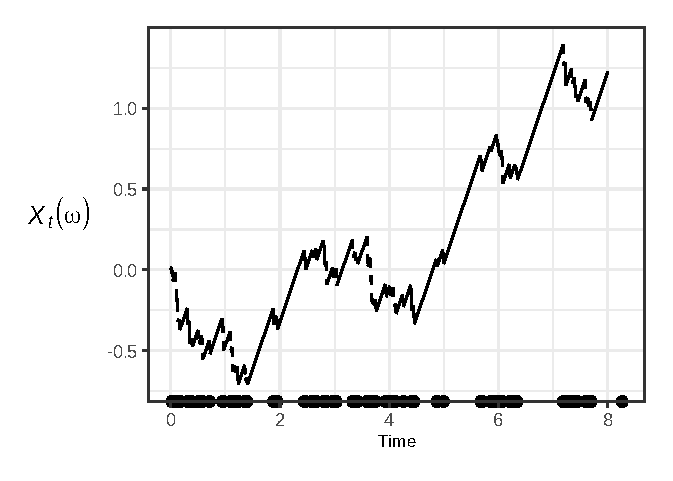
\includegraphics{input_prsnt}
\end{frame}


\begin{frame}{Simulated example: workload process}
  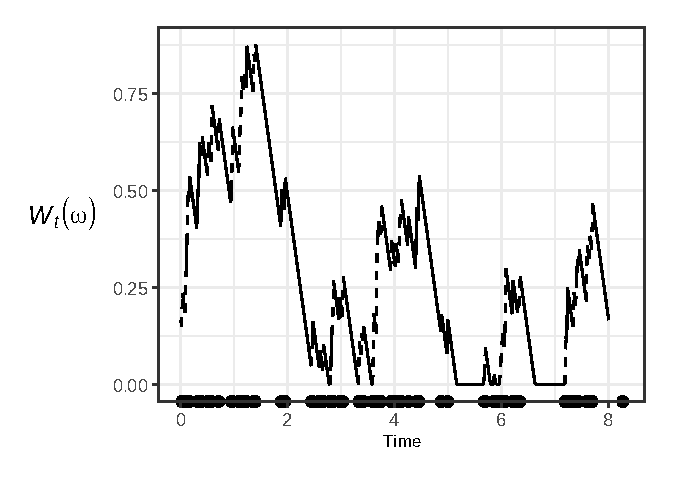
\includegraphics{workload_prsnt}
\end{frame}

\section{Idle time}

\begin{frame}{Total idle time}
  \begin{definition}
    The total idle time of a general storage model is the integral
    \begin{equation}
      I \coloneqq \int_{(0, +\infty)} \mathbbm{1}_{\{ W_t = 0 \}} dt \,.
    \end{equation}
  \end{definition}
\end{frame}

\begin{frame}{Total idle time}
  \begin{itemize}
    \item Measures the efficiency of the system
    \item Too large => resources not fully utilised
    \item Example: parallel computation with race conditions => worker threads in spinlock
    \item Distribution determined by $\lambda \mu$ (mean incoming work per unit time):
    \begin{itemize}
      \item $\lambda \mu \leq 1$ => queue repeatedly becomes empty
      \item $\lambda \mu > 1$ => eventually the queue never empties
    \end{itemize}
  \end{itemize}
\end{frame}


\begin{frame}{Distribution of $I$}
  \small
  \begin{theorem} \label{thm:pois-idle-time}
    Let $\{ W_t \}$ be the workload process of an $M/G/1$ queue with arrival rate $\lambda$ and service distribution $F$ satisfying $\EX[\mathbb{E}_F]{X} = \mu$, and consider the function
    \begin{equation}
      \psi(\theta) \coloneqq \theta - \lambda \int_{(0, \infty)} \left( 1 - e^{-\theta x} \right) F(dx)  \,,
    \end{equation}
    defined for $\theta \geq 0$. Then the following hold:
    \begin{enumerate}[(i)]
      \item \label{pois_idle_time-i}
      If $\mu \lambda \leq 1$, then $I = \infty$ a.s.
      \item \label{pois_idle_time-ii}
      If $\mu \lambda > 1$ and $\theta^*$ is the largest root of $\psi$, then
      \begin{equation}
        \prob_I = (1 - e^{-\theta^* w}) \delta_0 + \theta^* e^{-\theta^*{(w + x)}} \mathrm{Leb}
      \end{equation}
      where $\delta_0$ denotes the Dirac measure at $0$ and $\mathrm{Leb}$ is the Lebesgue measure.
    \end{enumerate}
  \end{theorem}
\end{frame}

\begin{frame}[plain]{Simulated example with $\lambda \mu \leq 1$: parameters}
  \begin{itemize}
    \item discrete grid $t_1, \dots, t_n$ with $t_1 = 0$, $t_n = 8$, $n = 480$ (samples every minute)
    \item $\lambda = 12$
    \item $\mu = 4 / 60 \approx 0.0667$
    \item $F \sim \Gamma(\frac{\mu^2}{\sigma^2}, \frac{\mu}{\sigma^2})$ with standard deviation $\sigma = 2.5 / 60 \approx 0.0417$ 
  \end{itemize}
\end{frame}

\begin{frame}[plain]{Simulated example with $\lambda \mu \leq 1$: input process}
  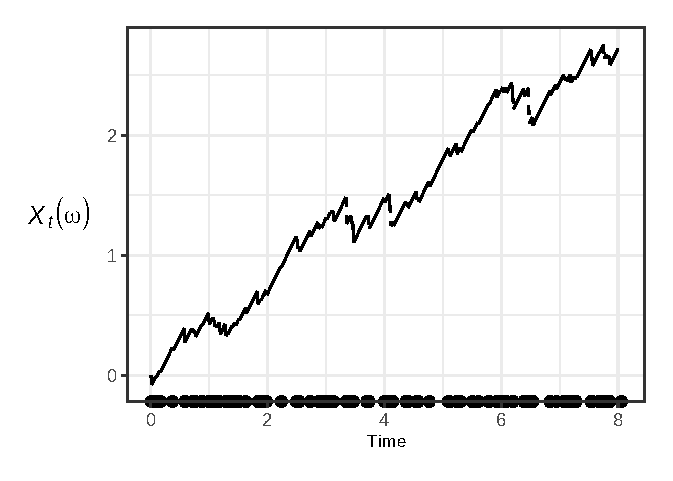
\includegraphics{input_leq_1_prsnt}
\end{frame}

\begin{frame}{Simulated example with $\lambda \mu \leq 1$: workload process}
  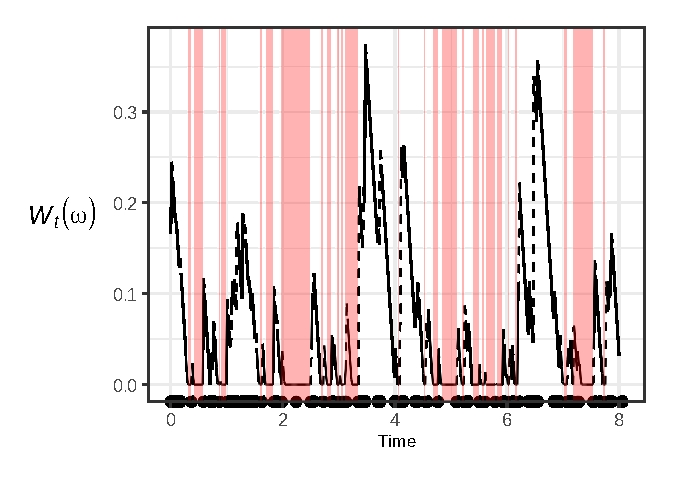
\includegraphics{workload_leq_1_prsnt}
\end{frame}

\begin{frame}[plain]{Simulated example with $\lambda \mu > 1$: parameters}
  \begin{itemize}
    \item discrete grid $t_1, \dots, t_n$ with $t_1 = 0$, $t_n = 8$, $n = 480$ (samples every minute)
    \item $\lambda = 12$
    \item $\mu = 6 / 60 = 0.1$
    \item $F \sim \Gamma(\frac{\mu^2}{\sigma^2}, \frac{\mu}{\sigma^2})$ with standard deviation $\sigma = 2.5 / 60 \approx 0.0417$ 
  \end{itemize}
\end{frame}

\begin{frame}[plain]{Simulated example with $\lambda \mu > 1$: input process}
  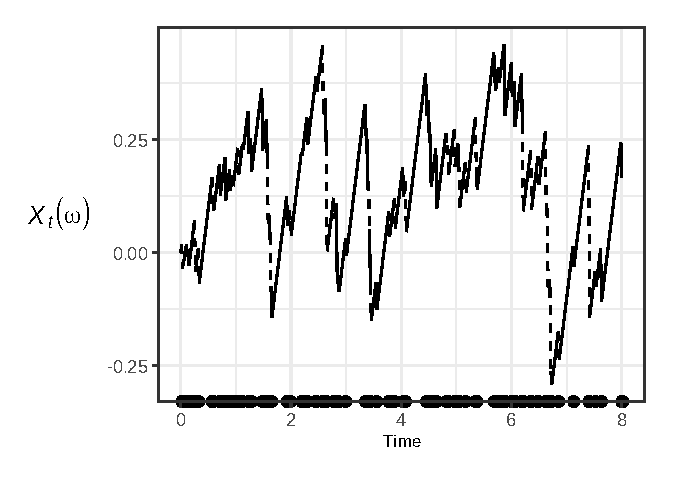
\includegraphics{input_ge_1_prsnt}
\end{frame}

\begin{frame}{Simulated example with $\lambda \mu > 1$: workload process}
  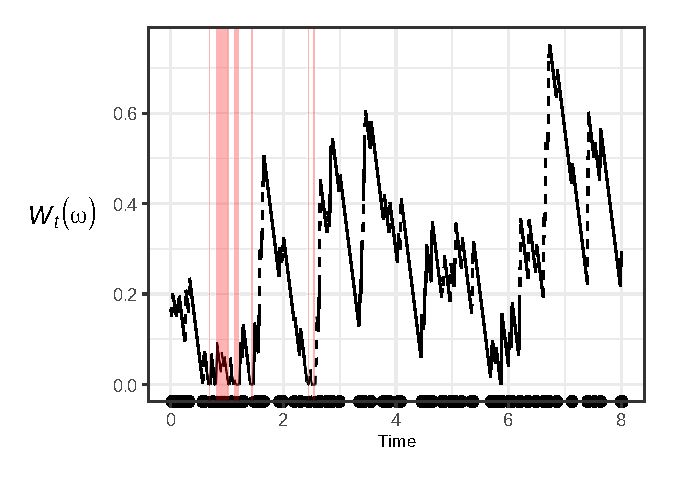
\includegraphics{workload_ge_1_prsnt}
\end{frame}

\begin{frame}{Proof outline}
  
\end{frame}

\begin{frame}[allowframebreaks]{References}
  \tiny
  \nocite{*}
  \printbibliography
\end{frame}

\end{document}